\documentclass[10pt,aspectratio=43]{beamer}
\usepackage{graphicx}
\usepackage{xcolor}
\usepackage{pgfplots}
\usepackage{tikz}
\usepackage[most]{tcolorbox}
\usepackage{booktabs}  % For professional table formatting
\pgfplotsset{compat=1.17}

% ========== Colors & Theme ==========
\definecolor{myMaroon}{RGB}{158, 27, 50}
\definecolor{myBlue}{RGB}{90, 27, 158}

\usetheme{CambridgeUS}
\setbeamercolor*{titlelike}{fg=myMaroon}

% ========== Title Page ==========
\title{Algorithms, Design \& Analysis}
\subtitle{Lecture 19: Dijkstra's Algorithm, Huffman Compression \\ \& Floyd-Warshall Algorithm}
\author[BSCS23008 \& BSCS23086]{Abdullah Hussain Yasim \& M. Ibrahim Butt}
\institute[ITU]{Information Technology University}
\date{April 11, 2025}

\begin{document}

\begin{frame}
    \titlepage
\end{frame}


\begin{frame}
    \frametitle{About Your Fellows}
    \begin{itemize}
        \item Hi there! We are \textbf{Abdullah Hussain Yasim} and \textbf{Muhammad Ibrahim Butt}.
        \item We are Associate Students at ITU.
    \end{itemize}
    
\end{frame}


\begin{frame}
    \frametitle{\textcolor{myMaroon}{Dijkstra’s Algorithm}}
    \begin{center}
        {\Large \textbf{\textcolor{myMaroon}{Dijkstra’s Algorithm}}} \\
        \vspace{0.3cm}
        {\large \textcolor{myBlue}{(Finding the Shortest Path in a Weighted Graph)}}
    \end{center}

    % Footer
\end{frame}


\begin{frame}
    \frametitle{Dijkstra's Algorithm}
    \begin{itemize}
        \item \textcolor{myMaroon}{\textbf{What is it?}}
        \begin{itemize}
            \item Dijkstra’s Algorithm is a greedy algorithm used to find the shortest path from a single source node to all other nodes in a weighted graph.
        \end{itemize}
        

        \vspace{0.3cm}
        \item \textcolor{myMaroon}{\textbf{Input/Output:}}
        \begin{itemize}
            \item Input: Graph, Start node
            \item Output: Shortest paths \& distances to all other nodes
        \end{itemize}


        \vspace{0.3cm}
        \item \textcolor{myMaroon}{\textbf{Characteristics:}}
        \begin{itemize}
            \item It gives better time complexity.
            \item It is greedy algorithm.
            \item Can work with negative weight edges (but can gives incorrect answer).
            \item Fails with negative cycles (Stuck in loop).
        \end{itemize}
        
    \end{itemize}

    % Footer

\end{frame}



\begin{frame}
    \frametitle{\textcolor{myMaroon}{Greedy Algorithms}}
    \begin{center}
        {\Large \textbf{\textcolor{myMaroon}{Greedy Algorithms}}} \\
        \vspace{0.3cm}
        {\large \textcolor{myBlue}{(Making the best local choice at every step)}}
    \end{center}

    % Footer
\end{frame}



\begin{frame}
    \frametitle{Greedy Algorithm}
    \begin{itemize}
    \item \textcolor{myMaroon}{\textbf{Definition:}}
    \begin{itemize}
        \item An algorithm that makes \textbf{locally optimal choices} at each step.
    \end{itemize}
        
        \vspace{0.5cm}
        \item \textcolor{myMaroon}{\textbf{Characteristics:}}
        \begin{itemize}
            \item Makes locally optimal choices at each step
            \item No backtracking
            \item Requires \textbf{greedy choice property} and \textbf{optimal substructure}
        \end{itemize}
        
        \vspace{0.5cm}
        \item \textcolor{myMaroon}{\textbf{Examples:}}
        \begin{itemize}
            \item Dijkstra’s Algorithm
            \item Minimum Spanning Tree (Prim’s, Kruskal’s)
            \item Huffman Compression
        \end{itemize}
        
        \vspace{0.5cm}
        \item \textcolor{red}{\textbf{Note:}} May not work for all problems (e.g., 0/1 Knapsack)
    \end{itemize}
    
    % Footer
\end{frame}




\begin{frame}
    \frametitle{Local Maximum Problem}
\begin{center}
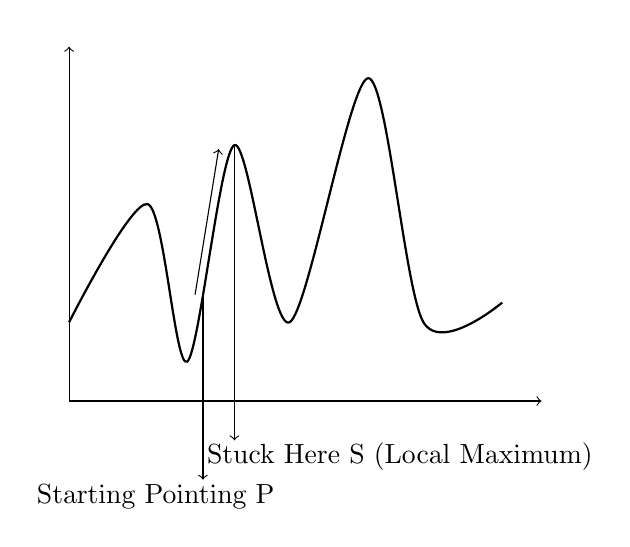
\begin{tikzpicture}
    % Axes
    \draw[->] (0,0) -- (6,0) node[right] {};
    \draw[->] (0,0) -- (0,4.5) node[above] {};
    
    % Wavy line
    \draw[thick, smooth] plot coordinates {(0,1) (1,2.5) (1.5,0.5) (2.1,3.25) (2.8,1) (3.8,4.1) (4.5,1) (5.5,1.25)};
    
    % Arrow pointing to peak
    \draw[->] (1.7,1.35) -- (1.7,-1);
    \draw[->] (2.1,3.25) -- (2.1,-0.5);
    \draw[->] (1.6,1.35) -- (1.9,3.2);
    
    % Annotation
    \node[above] at (1.1,-1.5) {Starting Pointing P};
    \node[above] at (4.2,-1) {Stuck Here S (Local Maximum)};
\end{tikzpicture}
\end{center}
\end{frame}



\begin{frame}
    \frametitle{Local Optimization Limitation}
  
    \begin{itemize}
        \item \textcolor{myMaroon}{\textbf{Process:}}
        \begin{itemize}
            \item Starts at point P, evaluates immediate neighbors (left/right).
            \item Always selects \textbf{best local move} (like hill-climbing)
            \item Gets stuck at point S if no better neighbors exist (local optimum).
        \end{itemize}

        \vspace{0.5cm}
        
        \item \textcolor{myMaroon}{\textbf{Why it fails:}}
        \begin{itemize}
            \item No memory of previous states (no backtracking).
            \item No knowledge of global landscape (only sees local).
            \item Works well only for convex problems.
        \end{itemize}

        \vspace{0.5cm}

         \item \textcolor{myMaroon}{\textbf{Note:}}
        \begin{itemize}
            \item Local maximum (or local optimum) problems do not occur in Dijkstra's Algorithm and MST algorithms (Prim’s, Kruskal’s) if all edge weights are positive.
        \end{itemize}

    \end{itemize}

    % Footer
\end{frame}






% ===== Slide 1: Title Slide =====
\begin{frame}
    \frametitle{\textcolor{myMaroon}{Types of Compression}}
    \begin{center}
        {\Large \textbf{\textcolor{myMaroon}{Types of Compression}}} \\
        \vspace{0.5cm}
        {\large \textcolor{myBlue}{Lossy vs Lossless Compression}}
    \end{center}

    % Footer
\end{frame}




% ===== Slide 2: What is Compression? =====
\begin{frame}
    \frametitle{\textcolor{myMaroon}{What is Compression?}}
    \begin{itemize}
        \item \textcolor{myMaroon}{\textbf{Definition:}} \\
        Process of reducing file size by encoding data more efficiently
        
        \vspace{0.5cm}
        \item \textcolor{myMaroon}{\textbf{Two Main Types:}}
        \begin{itemize}
            \item \textcolor{myBlue}{\textbf{Lossy Compression}} \\
            (Permanently removes some data)
            
            \item \textcolor{myBlue}{\textbf{Lossless Compression}} \\
            (Preserves all original data)
        \end{itemize}
    \end{itemize}

    % Footer

\end{frame}



% ===== Slide 3: Lossy Compression =====
\begin{frame}
    \frametitle{\textcolor{myMaroon}{Lossy Compression}}
    \begin{itemize}
        \item \textcolor{myMaroon}{\textbf{Definition:}} \\
        Compression where some data is discarded, leading to quality loss
        
        \vspace{0.4cm}
        \item \textcolor{myMaroon}{\textbf{Key Points:}}
        \begin{itemize}
            \item Irreversible (original data cannot be perfectly reconstructed)
            \item Prioritizes file size reduction over quality preservation
            \item Best for human-perceived media (audio/video/images)
        \end{itemize}
        
        \vspace{0.4cm}
        \item \textcolor{myMaroon}{\textbf{Examples:}}
        \begin{itemize}
            \item \textcolor{myBlue}{MP3} (Audio)
            \item \textcolor{myBlue}{JPEG} (Images)
            \item \textcolor{myBlue}{MPEG-4} (Video)
        \end{itemize}
    \end{itemize}

    % Footer

\end{frame}


% ===== Slide 4: Lossless Compression =====
\begin{frame}
    \frametitle{\textcolor{myMaroon}{Lossless Compression}}
    \begin{itemize}
        \item \textcolor{myMaroon}{\textbf{Definition:}} \\
        Compression with no data loss - exact original can be restored
        
        \vspace{0.4cm}
        \item \textcolor{myMaroon}{\textbf{Key Points:}}
        \begin{itemize}
            \item Fully reversible compression
            \item Maintains data integrity and accuracy
            \item Essential for sensitive/critical data
        \end{itemize}
        
        \vspace{0.4cm}
        \item \textcolor{myMaroon}{\textbf{Examples:}}
        \begin{itemize}
            \item \textcolor{myBlue}{ZIP} archives
            \item \textcolor{myBlue}{PNG} images
            \item \textcolor{myBlue}{Sensor data} storage
            \item \textcolor{myBlue}{Text documents}
        \end{itemize}
    \end{itemize}

    % Footer
\end{frame}


\begin{frame}
    \frametitle{\textcolor{myMaroon}{Summary}}
    \begin{columns}[T]
        % Left Column - Lossy
        \begin{column}{0.48\textwidth}
            \centering
            \textcolor{myMaroon}{\textbf{Lossy Compression}}
            \begin{itemize}
                \item Some data is permanently lost
                \item Cannot restore original exactly
                \item Smaller file sizes
                \item Best for: \\
                Audio (MP3), Video (MP4), Images (JPEG)
            \end{itemize}
        \end{column}
        
        % Right Column - Lossless
        \begin{column}{0.48\textwidth}
            \centering
            \textcolor{myMaroon}{\textbf{Lossless Compression}}
            \begin{itemize}
                \item No data loss
                \item Perfect reconstruction
                \item Larger file sizes
                \item Best for: \\
                Text, Code, Sensor data, Archives (ZIP)
            \end{itemize}
        \end{column}
    \end{columns}


    % Footer
\end{frame}



% ===== Slide 1: Title Slide =====
\begin{frame}
    \frametitle{\textcolor{myMaroon}{Huffman's Compression}}
    \begin{center}
        {\Large \textbf{\textcolor{myMaroon}{Huffman's Compression}}} \\
        \vspace{0.3cm}
        {\large \textcolor{myBlue}{(Lossless Encoding)}}
    \end{center}

    % Footer
\end{frame}



% ===== Slide 2: What is Huffman Compression? =====
\begin{frame}
    \frametitle{\textcolor{myMaroon}{What is Huffman Compression?}}
    \begin{itemize}
        \item A \textbf{lossless compression algorithm}
        
        \vspace{0.4cm}
        \item Reduces file size using \textbf{variable-length encoding}
        
        \vspace{0.4cm}
        \item Based on \textbf{frequency of characters}
        
        \vspace{0.4cm}
        \item \textbf{No data is lost}, and original can be perfectly reconstructed
    \end{itemize}

    % Footer
\end{frame}




% ===== Slide 3: Input/Output =====
\begin{frame}
    \frametitle{\textcolor{myMaroon}{Input/Output}}
    \begin{itemize}
        \item \textcolor{myMaroon}{\textbf{Input:}} 
        \begin{itemize}
            \item Text file or string
        \end{itemize}
        
        \vspace{0.5cm}
        \item \textcolor{myMaroon}{\textbf{Output:}} 
        \begin{itemize}
            \item Compressed binary text
            \item Huffman Tree or Lookup Table (for decoding)
        \end{itemize}
    \end{itemize}

    % Footer
\end{frame}


\begin{frame}
    \frametitle{\textcolor{myMaroon}{Key Characteristics}}

    \begin{itemize}
    \item \textcolor{myMaroon}{\textbf{Properties:}} 
    \begin{itemize}
        \item Lossless (reversible)
        \item Uses Priority Queue (Min-Heap)
        \item Shorter codes for frequent characters
        \item Optimal prefix code (no ambiguity in decoding)
        \item Prefix-free code: No code is the prefix of another
        \item Only leaf nodes contain characters
        \item Each character is initially represented as a singular-node tree, where:
        \begin{itemize}
            
            \item The node = character
            \item The weight = frequency of the character
            \end{itemize}
    \end{itemize}
    \end{itemize}
\end{frame}



\begin{frame}
    \frametitle{Steps of Huffman Algorithm}
    \begin{itemize}
    \item \textcolor{myMaroon}{\textbf{Steps:}} 
    \begin{itemize}
        \item Build frequency table of all characters
        \item Create nodes for each character
        \item Insert nodes into a min-heap (priority queue)
        \item Merge two nodes with the lowest frequency. The combined frequency is the sum of the two individual frequencies.
        \item Repeat until one tree remains
        \item Assign 0 to left, 1 to right during traversal
        \item Encode each character using its path in the tree
    \end{itemize}
    \end{itemize}
\end{frame}



\begin{frame}
    \frametitle{\textcolor{myMaroon}{Huffman Compression: Example}}
    
    \begin{itemize}
        \item \textcolor{myMaroon}{\textbf{Example:}}
        
        \vspace{0.3cm}
        \begin{itemize}
            \item \textcolor{myBlue}{Using the string:}
            
            \begin{center}
                \texttt{"the average cost of each operation in an algorithm when spread"}
            \end{center}
        \end{itemize}
    \end{itemize}
\end{frame}






% First Slide
\begin{frame}
    \frametitle{\textcolor{myMaroon}{Character Frequency Analysis (Part 1)}}

    
 \begin{itemize}
     \item \textcolor{myMaroon}{Frequency Table:}
\end{itemize}
    \begin{center}
        \begin{tabular}{c c}
            \toprule
            \textcolor{myMaroon}{\textbf{Character}} & \textcolor{myMaroon}{\textbf{Frequency}} \\
            \midrule
            a & 7 \\
            c & 2 \\
            e & 7 \\
            f & 1 \\
            g & 2 \\
            h & 4 \\
            i & 3 \\
            m & 1 \\
            n & 4 \\
            o & 5 \\
            \bottomrule
        \end{tabular}
    \end{center}
\end{frame}

% Second Slide
\begin{frame}
    \frametitle{\textcolor{myMaroon}{Character Frequency Analysis (Part 2)}}
    
    \begin{center}
        \begin{tabular}{c c}
            \toprule
            \textcolor{myMaroon}{\textbf{Character}} & \textcolor{myMaroon}{\textbf{Frequency}} \\
            \midrule
            p & 2 \\
            r & 4 \\
            s & 2 \\
            d & 1 \\
            t & 4 \\
            v & 1 \\
            w & 1 \\
            spaces & 10 \\
            \bottomrule
        \end{tabular}
    \end{center}

    
\end{frame}




\begin{frame}
    \frametitle{\textcolor{myMaroon}{Huffman Tree Example}}
    
    \begin{itemize}
        \setlength\itemsep{0pt} % Reduces space between items
        \setlength\parskip{0pt} % Reduces paragraph spacing
        \item Now using the min-heap, merge the singular node tree
    \end{itemize}
        \centering
        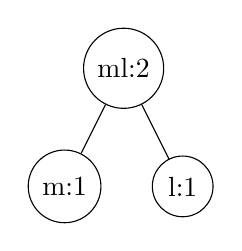
\begin{tikzpicture}[
            level distance=1.5cm,
            level 1/.style={sibling distance=1.5cm},
            every node/.style={draw, circle, minimum size=0.7cm}
        ]
        \node {ml:2}
            child { node {m:1} }
            child { node {l:1}};
        \end{tikzpicture}

 
\end{frame}








\begin{frame}
    \frametitle{\textcolor{myMaroon}{Huffman Tree Example}}

    
    \begin{columns}[T]
        % Left Tree
        \begin{column}{0.5\textwidth}
            \centering
            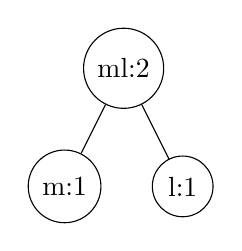
\begin{tikzpicture}[
                level distance=1.5cm,
                level 1/.style={sibling distance=1.5cm},
                every node/.style={draw, circle, minimum size=0.7cm}
            ]
            \node {ml:2}
                child { node {m:1}}
                child { node {l:1}};
            \end{tikzpicture}
        \end{column}

        % Right Tree
        \begin{column}{0.5\textwidth}
            \centering
            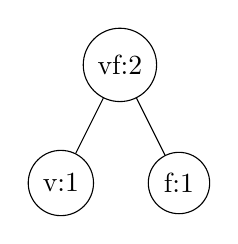
\begin{tikzpicture}[
                level distance=1.5cm,
                level 1/.style={sibling distance=1.5cm},
                every node/.style={draw, circle, minimum size=0.7cm}
            ]
            \node {vf:2}
                child { node {v:1}}
                child { node {f:1} };
            \end{tikzpicture}
        \end{column}
    \end{columns}


\end{frame}



\begin{frame}
    \frametitle{\textcolor{myMaroon}{Huffman Tree Example}}
    
    \begin{columns}[T]
        % Left Tree
        \begin{column}{0.33\textwidth}
            \centering
            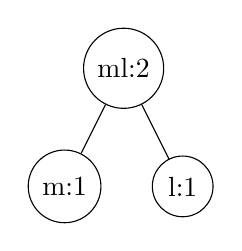
\begin{tikzpicture}[
                level distance=1.5cm,
                level 1/.style={sibling distance=1.5cm},
                every node/.style={draw, circle, minimum size=0.7cm}
            ]
            \node {ml:2}
                child { node {m:1}}
                child { node {l:1}};
            \end{tikzpicture}
        \end{column}

        % Right Tree
        \begin{column}{0.33\textwidth}
            \centering
            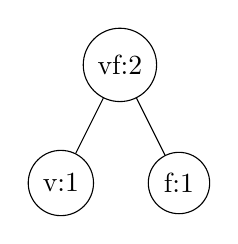
\begin{tikzpicture}[
                level distance=1.5cm,
                level 1/.style={sibling distance=1.5cm},
                every node/.style={draw, circle, minimum size=0.7cm}
            ]
            \node {vf:2}
                child { node {v:1}}
                child { node {f:1} };
            \end{tikzpicture}
        \end{column}

        \begin{column}{0.33\textwidth}
            \centering
            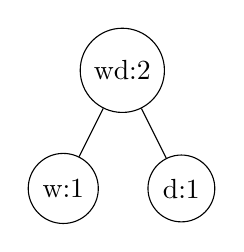
\begin{tikzpicture}[
                level distance=1.5cm,
                level 1/.style={sibling distance=1.5cm},
                every node/.style={draw, circle, minimum size=0.7cm}
            ]
            \node {wd:2}
                child { node {w:1}}
                child { node {d:1} };
            \end{tikzpicture}
        \end{column}
        
    \end{columns}


\end{frame}



\begin{frame}
    \frametitle{\textcolor{myMaroon}{Huffman Tree Example}}
    \begin{columns}[T]
        % Tree 1
        \begin{column}{0.33\textwidth}
            \centering
            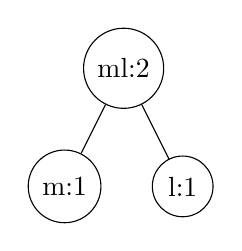
\begin{tikzpicture}[
                level distance=1.5cm,
                level 1/.style={sibling distance=1.5cm},
                every node/.style={draw, circle, minimum size=0.7cm}
            ]
            \node {ml:2}
                child { node {m:1} }
                child { node {l:1} };
            \end{tikzpicture}
        \end{column}

        % Tree 2
        \begin{column}{0.33\textwidth}
            \centering
            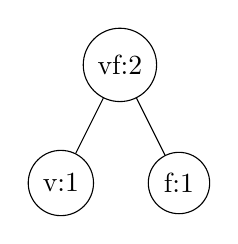
\begin{tikzpicture}[
                level distance=1.5cm,
                level 1/.style={sibling distance=1.5cm},
                every node/.style={draw, circle, minimum size=0.7cm}
            ]
            \node {vf:2}
                child { node {v:1} }
                child { node {f:1} };
            \end{tikzpicture}
        \end{column}

        % Tree 3
        \begin{column}{0.33\textwidth}
            \centering
            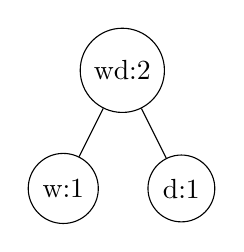
\begin{tikzpicture}[
                level distance=1.5cm,
                level 1/.style={sibling distance=1.5cm},
                every node/.style={draw, circle, minimum size=0.7cm}
            ]
            \node {wd:2}
                child { node {w:1} }
                child { node {d:1} };
            \end{tikzpicture}
        \end{column}
    \end{columns}

    \vspace{1cm} % Space between rows
    
    % Tree 4 (Second Row)
    \begin{center}
        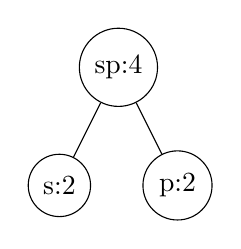
\begin{tikzpicture}[
            level distance=1.5cm,
            level 1/.style={sibling distance=1.5cm},
            every node/.style={draw, circle, minimum size=0.7cm}
        ]
        \node {sp:4}
            child { node {s:2} }
            child { node {p:2} };
        \end{tikzpicture} % Fixed typo here
    \end{center}
\end{frame}


\begin{frame}
    \frametitle{\textcolor{myMaroon}{Huffman Tree Example}}
    \begin{columns}[T]
        % Tree 1
        \begin{column}{0.33\textwidth}
            \centering
            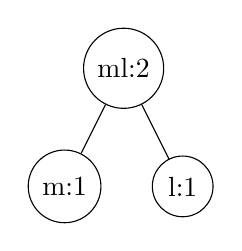
\begin{tikzpicture}[
                level distance=1.5cm,
                level 1/.style={sibling distance=1.5cm},
                every node/.style={draw, circle, minimum size=0.7cm}
            ]
            \node {ml:2}
                child { node {m:1} }
                child { node {l:1} };
            \end{tikzpicture}
        \end{column}

        % Tree 2
        \begin{column}{0.33\textwidth}
            \centering
            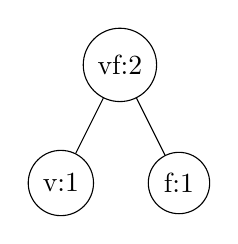
\begin{tikzpicture}[
                level distance=1.5cm,
                level 1/.style={sibling distance=1.5cm},
                every node/.style={draw, circle, minimum size=0.7cm}
            ]
            \node {vf:2}
                child { node {v:1} }
                child { node {f:1} };
            \end{tikzpicture}
        \end{column}

        % Tree 3
        \begin{column}{0.33\textwidth}
            \centering
            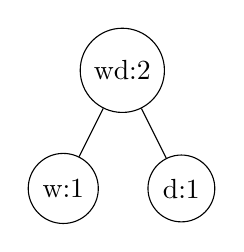
\begin{tikzpicture}[
                level distance=1.5cm,
                level 1/.style={sibling distance=1.5cm},
                every node/.style={draw, circle, minimum size=0.7cm}
            ]
            \node {wd:2}
                child { node {w:1} }
                child { node {d:1} };
            \end{tikzpicture}
        \end{column}
    \end{columns}

    \vspace{1cm} % Space between rows
    
    % Tree 4 (Second Row)
    \begin{columns}[T]
        % Tree 1
        \begin{column}{0.5\textwidth}
            \centering
            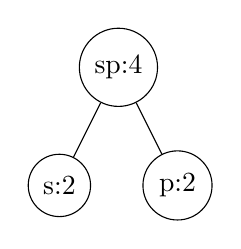
\begin{tikzpicture}[
                level distance=1.5cm,
                level 1/.style={sibling distance=1.5cm},
                every node/.style={draw, circle, minimum size=0.7cm}
            ]
            \node {sp:4}
                child { node {s:2} }
                child { node {p:2} };
            \end{tikzpicture}
        \end{column}

        % Tree 2
        \begin{column}{0.5\textwidth}
            \centering
            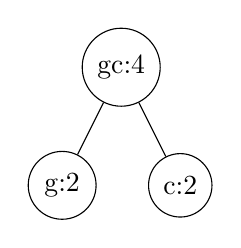
\begin{tikzpicture}[
                level distance=1.5cm,
                level 1/.style={sibling distance=1.5cm},
                every node/.style={draw, circle, minimum size=0.7cm}
            ]
            \node {gc:4}
                child { node {g:2} }
                child { node {c:2} };
            \end{tikzpicture}
        \end{column}

    \end{columns}
\end{frame}





% First Slide
\begin{frame}
    \frametitle{\textcolor{myMaroon}{Character Merge Tracking Table}}
    
    \begin{center}
        \begin{tabular}{c c c}
            \toprule
            \textcolor{myMaroon}{\textbf{Character/Node}} & 
            \textcolor{myMaroon}{\textbf{Frequency}} & 
            \textcolor{myMaroon}{\textbf{Used in Merge}} \\
            \midrule
            m & 1 & \checkmark \\[0.2cm]
            l & 1 & \checkmark \\[0.2cm]
            v & 1 & \checkmark \\[0.2cm]
            f & 1 & \checkmark \\[0.2cm]
            w & 1 & \checkmark \\[0.2cm]
            d & 1 & \checkmark \\[0.2cm]
            s & 2 & \checkmark \\[0.2cm]
            p & 2 & \checkmark \\[0.2cm]
            g & 2 & \checkmark \\[0.2cm]
            c & 2 & \checkmark \\[0.2cm]
            \bottomrule
        \end{tabular}
    \end{center}
\end{frame}








\begin{frame}
    \frametitle{\textcolor{myMaroon}{Huffman Tree Example}}
    
    \centering
    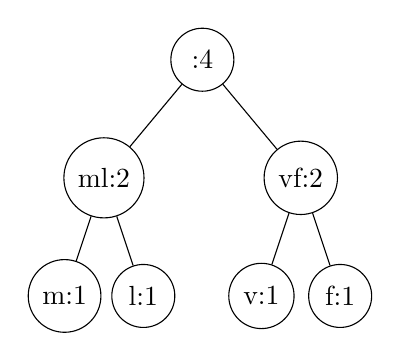
\begin{tikzpicture}[
        level distance=1.5cm,
        level 1/.style={sibling distance=2.5cm},
        level 2/.style={sibling distance=1cm},
        every node/.style={draw, circle, minimum size=0.8cm}
    ]
        \node {:4}
            child {
                node {ml:2}
                    child { node {m:1} }
                    child { node {l:1} }
            }
            child {
                node {vf:2}
                    child { node {v:1} }
                    child { node {f:1} }
            };
    \end{tikzpicture}
    
\end{frame}



\begin{frame}
    \frametitle{\textcolor{myMaroon}{Huffman Tree Example}}
    
    \centering
    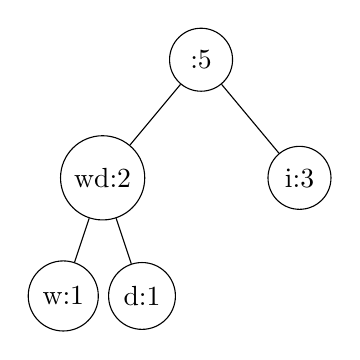
\begin{tikzpicture}[
        level distance=1.5cm,
        level 1/.style={sibling distance=2.5cm},
        level 2/.style={sibling distance=1cm},
        every node/.style={draw, circle, minimum size=0.8cm}
    ]
        \node {:5}
            child {
                node {wd:2}
                    child { node {w:1} }
                    child { node {d:1} }
            }
            child {
                node {i:3}
            };
    \end{tikzpicture}
    
\end{frame}


\begin{frame}
    \frametitle{\textcolor{myMaroon}{Huffman Tree Example}}
    \begin{columns}[T]
        % Tree 1
        \begin{column}{0.5\textwidth}
            \centering
    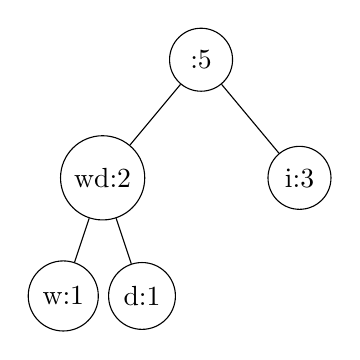
\begin{tikzpicture}[
        level distance=1.5cm,
        level 1/.style={sibling distance=2.5cm},
        level 2/.style={sibling distance=1cm},
        every node/.style={draw, circle, minimum size=0.8cm}
    ]
        \node {:5}
            child {
                node {wd:2}
                    child { node {w:1} }
                    child { node {d:1} }
            }
            child {
                node {i:3}
            };
    \end{tikzpicture}
        \end{column}

        % Tree 2
        \begin{column}{0.5\textwidth}
            \centering
            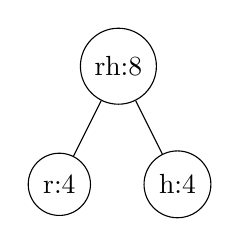
\begin{tikzpicture}[
                level distance=1.5cm,
                level 1/.style={sibling distance=1.5cm},
                every node/.style={draw, circle, minimum size=0.7cm}
            ]
            \node {rh:8}
                child { node {r:4} }
                child { node {h:4} };
            \end{tikzpicture}
        \end{column}

    \end{columns}

\end{frame}


\begin{frame}
    \frametitle{\textcolor{myMaroon}{Huffman Tree Example}}
    \begin{columns}[T]
        % Tree 1
        \begin{column}{0.33\textwidth}
            \centering
    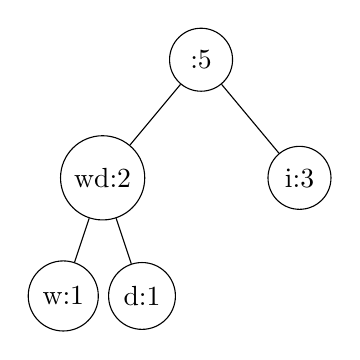
\begin{tikzpicture}[
        level distance=1.5cm,
        level 1/.style={sibling distance=2.5cm},
        level 2/.style={sibling distance=1cm},
        every node/.style={draw, circle, minimum size=0.8cm}
    ]
        \node {:5}
            child {
                node {wd:2}
                    child { node {w:1} }
                    child { node {d:1} }
            }
            child {
                node {i:3}
            };
    \end{tikzpicture}
        \end{column}

        % Tree 2
        \begin{column}{0.33\textwidth}
            \centering
            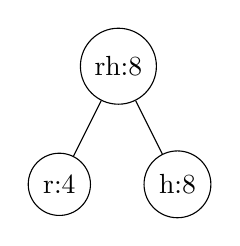
\begin{tikzpicture}[
                level distance=1.5cm,
                level 1/.style={sibling distance=1.5cm},
                every node/.style={draw, circle, minimum size=0.7cm}
            ]
            \node {rh:8}
                child { node {r:4} }
                child { node {h:8} };
            \end{tikzpicture}
        \end{column}


        %tree 3
        \begin{column}{0.33\textwidth}
            \centering
            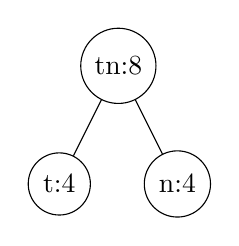
\begin{tikzpicture}[
                level distance=1.5cm,
                level 1/.style={sibling distance=1.5cm},
                every node/.style={draw, circle, minimum size=0.7cm}
            ]
            \node {tn:8}
                child { node {t:4} }
                child { node {n:4} };
            \end{tikzpicture}
        \end{column}

    \end{columns}

\end{frame}



\begin{frame}
    \frametitle{\textcolor{myMaroon}{Huffman Tree Example}}
    
    \centering
    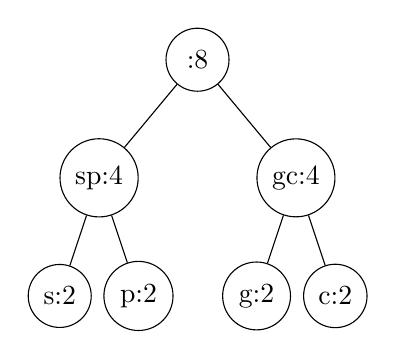
\begin{tikzpicture}[
        level distance=1.5cm,
        level 1/.style={sibling distance=2.5cm},
        level 2/.style={sibling distance=1cm},
        every node/.style={draw, circle, minimum size=0.8cm}
    ]
        \node {:8}
            child {
                node {sp:4}
                    child { node {s:2} }
                    child { node {p:2} }
            }
            child {
                node {gc:4}
                    child { node {g:2} }
                    child { node {c:2} }
            };
    \end{tikzpicture}
    
\end{frame}



\begin{frame}
    \frametitle{\textcolor{myMaroon}{Huffman Tree Example}}
    \centering
    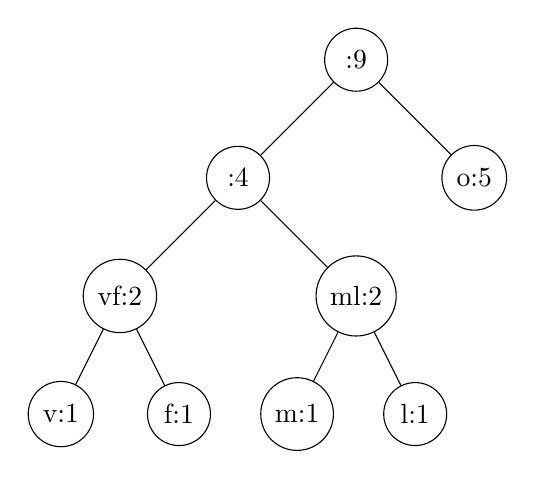
\begin{tikzpicture}[
        level distance=1.5cm,
        level 1/.style={sibling distance=3cm},
        level 2/.style={sibling distance=3cm},
        level 3/.style={sibling distance=1.5cm},
        every node/.style={draw, circle, minimum size=0.8cm}
    ]
        \node {:9}
            child {
                node {:4}
                    child {
                        node {vf:2}
                            child {node {v:1}}
                            child {node {f:1}}
                    }
                    child {
                        node {ml:2}
                            child {node {m:1}}
                            child {node {l:1}}
                    }
            }
            child {
                node {o:5}
            };
    \end{tikzpicture}
\end{frame}



\begin{frame}
    \frametitle{\textcolor{myMaroon}{Huffman Tree Example}}
    \centering
    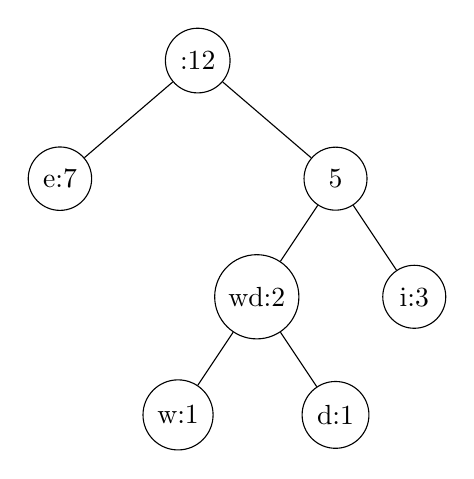
\begin{tikzpicture}[
        level distance=1.5cm,
        level 1/.style={sibling distance=3.5cm},
        level 2/.style={sibling distance=2cm},
        every node/.style={draw, circle, minimum size=0.8cm}
    ]
        \node {:12}
            child {
                node {e:7}
            }
            child {
                node {5}
                    child {
                        node {wd:2}
                            child {node {w:1}}
                            child {node {d:1}}
                    }
                    child {
                        node {i:3}
                    }
            };
    \end{tikzpicture}
\end{frame}



% First Slide
\begin{frame}
    \frametitle{\textcolor{myMaroon}{Character Merge Tracking Table}}
    
    \begin{center}
        \begin{tabular}{c c c}
            \toprule
            \textcolor{myMaroon}{\textbf{Character/Node}} & 
            \textcolor{myMaroon}{\textbf{Frequency}} & 
            \textcolor{myMaroon}{\textbf{Used in Merge}} \\
            \midrule
            m & 1 & \checkmark \\[0.2cm]
            l & 1 & \checkmark \\[0.2cm]
            v & 1 & \checkmark \\[0.2cm]
            f & 1 & \checkmark \\[0.2cm]
            w & 1 & \checkmark \\[0.2cm]
            d & 1 & \checkmark \\[0.2cm]
            s & 2 & \checkmark \\[0.2cm]
            p & 2 & \checkmark \\[0.2cm]
            g & 2 & \checkmark \\[0.2cm]
            c & 2 & \checkmark \\[0.2cm]
            
            %\bottomrule
        \end{tabular}
    \end{center}
\end{frame}


\begin{frame}
    \frametitle{\textcolor{myMaroon}{Character Merge Tracking Table}}
    
    \begin{center}
        \begin{tabular}{c c c}
            \toprule
            \textcolor{myMaroon}{\textbf{Character/Node}} & 
            \textcolor{myMaroon}{\textbf{Frequency}} & 
            \textcolor{myMaroon}{\textbf{Used in Merge}} \\
            \midrule
            i & 3 & \checkmark \\[0.2cm]
            r & 4 & \checkmark \\[0.2cm]
            h & 4 & \checkmark \\[0.2cm]
            t & 4 & \checkmark \\[0.2cm]
            n & 4 & \checkmark \\[0.2cm]
            o & 5 & \checkmark \\[0.2cm]
            e & 7 & \checkmark \\[0.2cm]
            
            \bottomrule
        \end{tabular}
    \end{center}
\end{frame}

\begin{frame}
    \frametitle{\textcolor{myMaroon}{Huffman Tree Combination Example}}

    \centering
    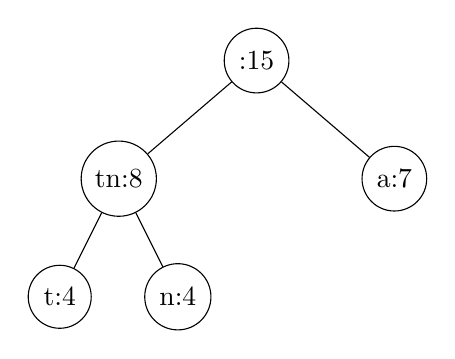
\begin{tikzpicture}[
        level distance=1.5cm,
        level 1/.style={sibling distance=3.5cm},
        level 2/.style={sibling distance=1.5cm},
        every node/.style={draw, circle, minimum size=0.8cm}
    ]
        \node {:15}
            child {
                node {tn:8}
                    child { node {t:4} }
                    child { node {n:4} }
            }
            child {
                node {a:7}
            };
    \end{tikzpicture}

\end{frame}

\begin{frame}
    \frametitle{\textcolor{myMaroon}{Huffman Tree Combination Example}}

    \centering
    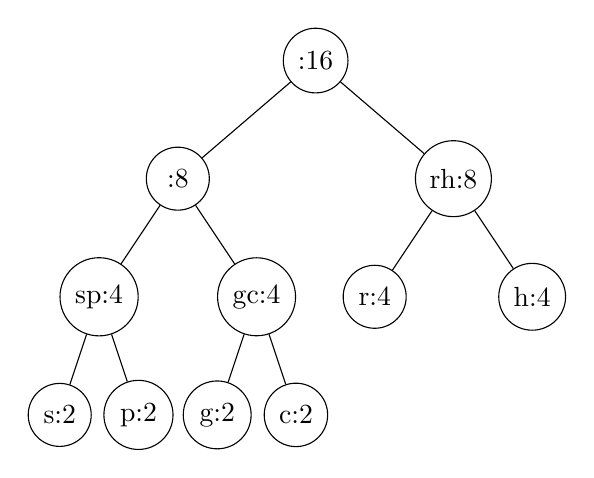
\begin{tikzpicture}[
        level distance=1.5cm,
        level 1/.style={sibling distance=3.5cm},
        level 2/.style={sibling distance=2cm},
        level 3/.style={sibling distance=1cm},
        every node/.style={draw, circle, minimum size=0.8cm}
    ]
        \node {:16}
            child {
                node {:8}
                    child {
                        node {sp:4}
                            child { node {s:2} }
                            child { node {p:2} }
                    }
                    child {
                        node {gc:4}
                            child { node {g:2} }
                            child { node {c:2} }
                    }
            }
            child {
                node {rh:8}
                    child { node {r:4} }
                    child { node {h:4} }
            };
    \end{tikzpicture}

\end{frame}

\begin{frame}
    \frametitle{\textcolor{myMaroon}{Huffman Tree Combination Example}}

    \centering
    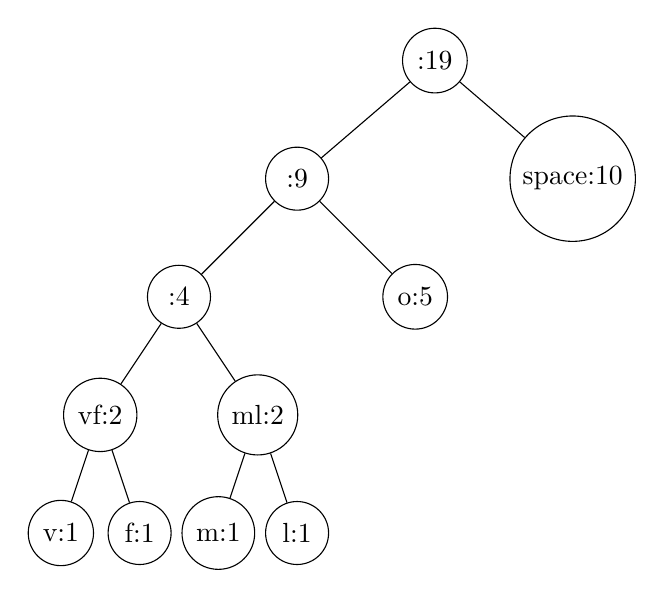
\begin{tikzpicture}[
        level distance=1.5cm,
        level 1/.style={sibling distance=3.5cm},
        level 2/.style={sibling distance=3cm},
        level 3/.style={sibling distance=2.cm},
        level 4/.style={sibling distance=1.0cm},
        every node/.style={draw, circle, minimum size=0.8cm}
    ]
        \node {:19}
            child {
                node {:9}
                    child {
                        node {:4}
                            child {
                                node {vf:2}
                                    child {node {v:1}}
                                    child {node {f:1}}
                            }
                            child {
                                node {ml:2}
                                    child {node {m:1}}
                                    child {node {l:1}}
                            }
                    }
                    child {
                        node {o:5}
                    }
            }
            child {
                node {space:10}
            };
    \end{tikzpicture}
\end{frame}


\begin{frame}
    \frametitle{\textcolor{myMaroon}{Character Merge Tracking Table}}
    
    \begin{center}
        \begin{tabular}{c c c}
            \toprule
            \textcolor{myMaroon}{\textbf{Character/Node}} & 
            \textcolor{myMaroon}{\textbf{Frequency}} & 
            \textcolor{myMaroon}{\textbf{Used in Merge}} \\
            \midrule
            m & 1 & \checkmark \\[0.2cm]
            l & 1 & \checkmark \\[0.2cm]
            v & 1 & \checkmark \\[0.2cm]
            f & 1 & \checkmark \\[0.2cm]
            w & 1 & \checkmark \\[0.2cm]
            d & 1 & \checkmark \\[0.2cm]
            s & 2 & \checkmark \\[0.2cm]
            p & 2 & \checkmark \\[0.2cm]
            g & 2 & \checkmark \\[0.2cm]
            c & 2 & \checkmark \\[0.2cm]
            
            %\bottomrule
        \end{tabular}
    \end{center}
\end{frame}

\begin{frame}
    \frametitle{\textcolor{myMaroon}{Character Merge Tracking Table}}
    
    \begin{center}
        \begin{tabular}{c c c}
            \toprule
            \textcolor{myMaroon}{\textbf{Character/Node}} & 
            \textcolor{myMaroon}{\textbf{Frequency}} & 
            \textcolor{myMaroon}{\textbf{Used in Merge}} \\
            \midrule
            i & 3 & \checkmark \\[0.2cm]
            r & 4 & \checkmark \\[0.2cm]
            h & 4 & \checkmark \\[0.2cm]
            t & 4 & \checkmark \\[0.2cm]
            n & 4 & \checkmark \\[0.2cm]
            o & 5 & \checkmark \\[0.2cm]
            e & 7 & \checkmark \\[0.2cm]
            a & 7 & \checkmark \\[0.2cm]
            space & 10 & \checkmark \\[0.2cm]
            \bottomrule
        \end{tabular}
    \end{center}
\end{frame}


\begin{frame}
    \frametitle{\textcolor{myMaroon}{Huffman Tree Combination Example}}

    \centering
    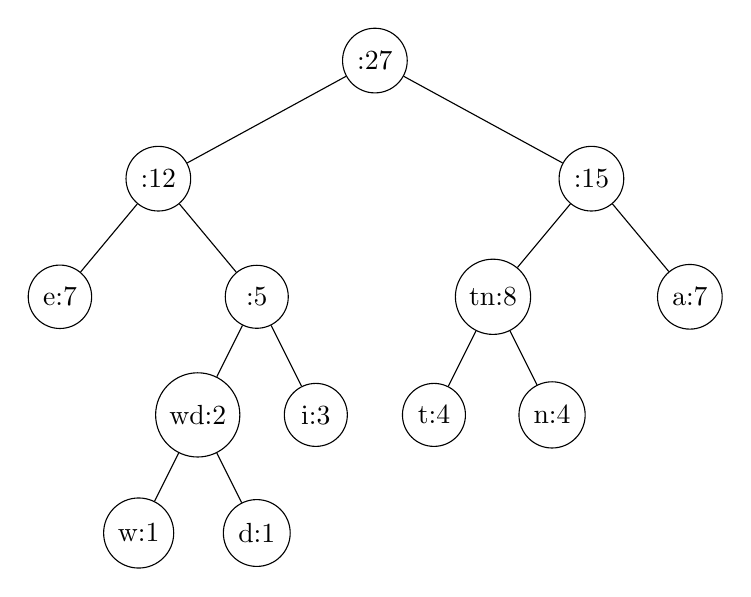
\begin{tikzpicture}[
        level distance=1.5cm,
        level 1/.style={sibling distance=5.5cm},
        level 2/.style={sibling distance=2.5cm},
        level 3/.style={sibling distance=1.5cm},
        every node/.style={draw, circle, minimum size=0.8cm}
    ]
        \node {:27}
            child {
                node {:12}
                    child {
                        node {e:7}
                    }
                    child {
                        node {:5}
                            child {
                                node {wd:2}
                                    child {node {w:1}}
                                    child {node {d:1}}
                            }
                            child {
                                node {i:3}
                            }
                    }
            }
            child {
                node {:15}
                    child {
                        node {tn:8}
                            child { node {t:4} }
                            child { node {n:4} }
                    }
                    child {
                        node {a:7}
                    }
            };
    \end{tikzpicture}
\end{frame}


\begin{frame}
    \frametitle{\textcolor{myMaroon}{Huffman Tree Combination Example}}

    \centering
    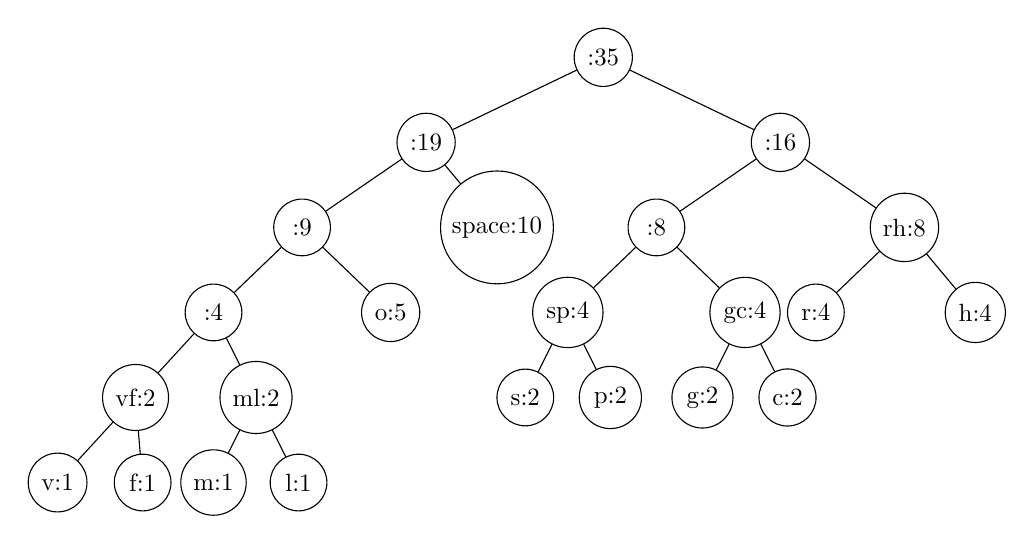
\begin{tikzpicture}[
        scale=0.9,
        transform shape,
        level distance=1.2cm,
        level 1/.style={sibling distance=5cm},
        level 2/.style={sibling distance=3.5cm},
        level 3/.style={sibling distance=2.5cm},
        level 4/.style={sibling distance=1.2cm},
        every node/.style={draw, circle, minimum size=0.8cm}
    ]
        \node {:35}
            child {
                node {:19}
                    child {
                        node {:9}
                            child {
                                node {:4}
                                    child [sibling distance=2.2cm] {
                                        node {vf:2}
                                            child {node {v:1}}
                                            child [sibling distance=0.2cm] {node {f:1}}
                                    }
                                    child {
                                        node {ml:2}
                                            child {node {m:1}}
                                            child {node {l:1}}
                                    }
                            }
                            child {
                                node {o:5}
                            }
                    }
                    child [sibling distance=2.0cm] {
                        node {space:10}
                    }
            }
            child {
                node {:16}
                    child {
                        node {:8}
                            child {
                                node {sp:4}
                                    child { node {s:2} }
                                    child { node {p:2} }
                            }
                            child {
                                node {gc:4}
                                    child { node {g:2} }
                                    child { node {c:2} }
                            }
                    }
                    child {
                        node {rh:8}
                            child { node {r:4} }
                            child [sibling distance=2.0cm] { node {h:4} }
                    }
            };
    \end{tikzpicture}
\end{frame}


\begin{frame}
    \frametitle{\textcolor{myMaroon}{Final Huffman Tree}}

    \centering
    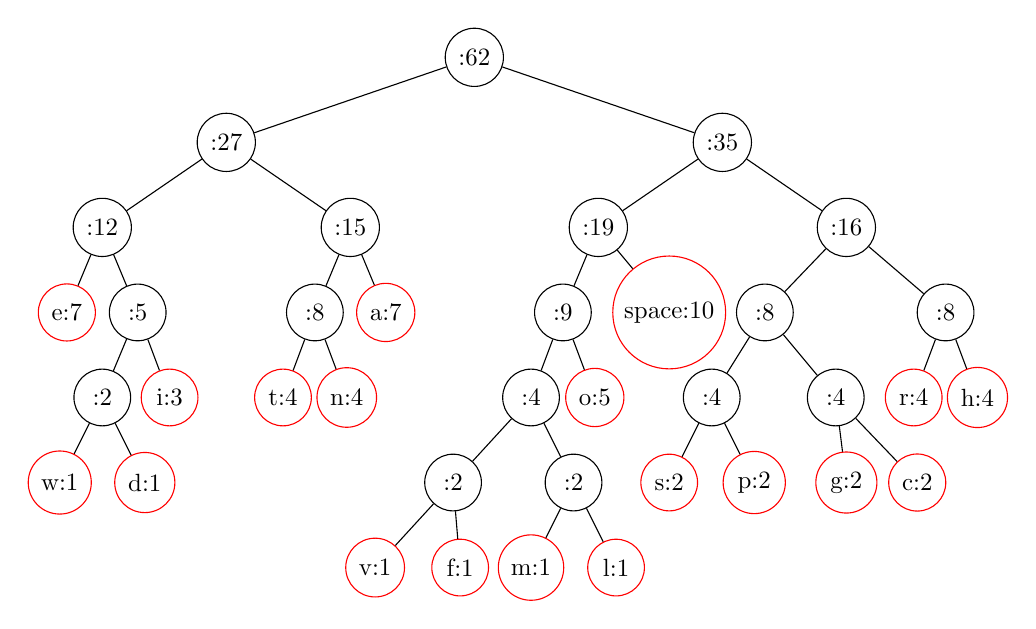
\begin{tikzpicture}[
        scale=0.9,
        transform shape,
        level distance=1.2cm,
        level 1/.style={sibling distance=7cm},
        level 2/.style={sibling distance=3.5cm},
        level 3/.style={sibling distance=1.0cm},
        level 4/.style={sibling distance=0.9cm},
        level 5/.style={sibling distance=1.2cm},
        every node/.style={draw, circle, minimum size=0.8cm}
    ]
        \node {:62}
            child {
                node {:27}
                    child {
                        node {:12}
                            child {
                                node [draw=red] {e:7}
                            }
                            child {
                                node {:5}
                                    child [sibling distance=1.0cm] {
                                        node {:2}
                                            child {node [draw=red] {w:1}}
                                            child {node [draw=red] {d:1}}
                                    }
                                    child {
                                        node [draw=red] {i:3}
                                    }
                            }
                    }
                    child {
                        node {:15}
                            child {
                                node {:8}
                                    child { node [draw=red] {t:4} }
                                    child { node [draw=red] {n:4} }
                            }
                            child {
                                node [draw=red] {a:7}
                            }
                    }
            }
            child {
                node {:35}
                    child {
                        node {:19}
                            child {
                                node {:9}
                                    child {
                                        node {:4}
                                            child [sibling distance=2.2cm] {
                                                node {:2}
                                                    child {node [draw=red] {v:1}}
                                                    child [sibling distance=0.2cm] {node [draw=red] {f:1}}
                                            }
                                            child {
                                                node {:2}
                                                    child {node [draw=red] {m:1}}
                                                    child {node [draw=red] {l:1}}
                                            }
                                    }
                                    child {
                                        node [draw=red] {o:5}
                                    }
                            }
                            child [sibling distance=2.0cm] {
                                node [draw=red] {space:10}
                            }
                    }
                    child {
                        node {:16}
                            child [sibling distance=2.3cm] {
                                node {:8}
                                    child [sibling distance=1.5cm] {
                                        node {:4}
                                            child { node [draw=red] {s:2} }
                                            child { node [draw=red] {p:2} }
                                    }
                                    child [sibling distance=2.0cm] {
                                        node {:4}
                                            child [sibling distance=-0.3cm] { node [draw=red] {g:2} }
                                            child [sibling distance=2.3cm] { node [draw=red] {c:2} }
                                    }
                            }
                            child [sibling distance=2.8cm]  {
                                node {:8}
                                    child { node [draw=red] {r:4} }
                                    child { node [draw=red] {h:4} }
                            }
                    }
            };
    \end{tikzpicture}
\end{frame}


\begin{frame}
    \frametitle{\textcolor{myMaroon}{Huffman Tree}}
    \begin{itemize}
        \item Assigning 1 to the right traversal of each node
        
        \vspace{0.4cm}
        \item Assigning 0 to the left traversal of each node
        
        \vspace{0.4cm}
        \item We will traverse through the tree and set the traversal binary code as the encoding of the character.
        
        \vspace{0.4cm}
        \item Doing so will assign smaller binary codes to more frequently occuring characters and larger binary codes to less frequent characters.

        \vspace{0.4cm}
        \item For example The binary code for \textbf{a} will be 011 and for \textbf{v} will be 100000
    \end{itemize}

    % Footer
\end{frame}

\begin{frame}
    \frametitle{\textcolor{myMaroon}{Final Huffman Tree}}

    \centering
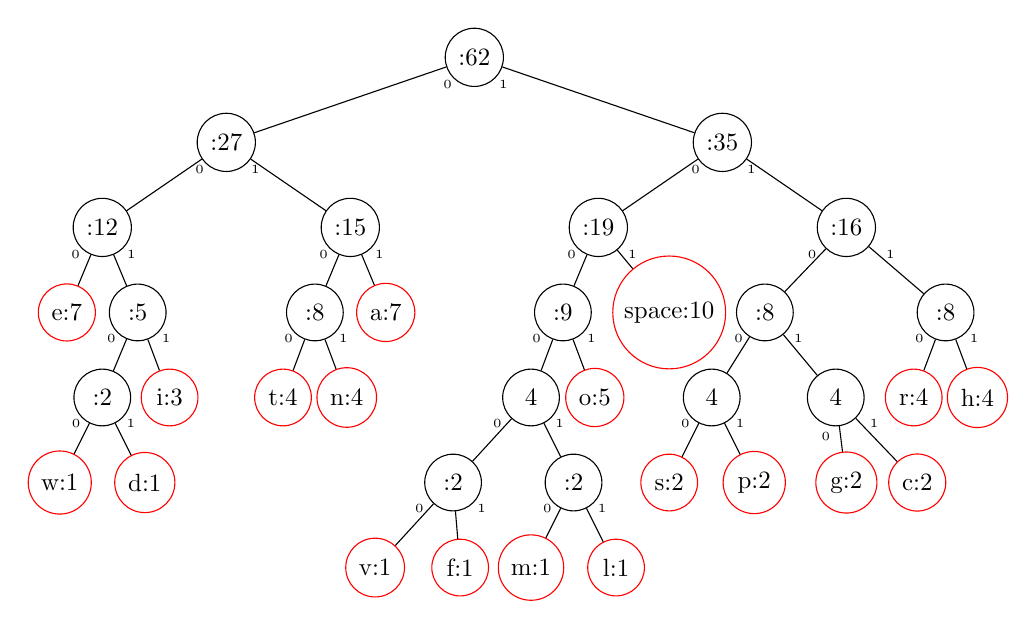
\begin{tikzpicture}[
    scale=0.9,
    transform shape,
    level distance=1.2cm,
    level 1/.style={sibling distance=7cm},
    level 2/.style={sibling distance=3.5cm},
    level 3/.style={sibling distance=1.0cm},
    level 4/.style={sibling distance=0.9cm},
    level 5/.style={sibling distance=1.2cm},
    code label/.style={
        font=\tiny\strut,       % Ensures consistent height
        inner sep=0pt,          % No padding
        text width=2.5pt,       % Minimal width
        minimum height=0pt,     % No extra height
        anchor=center           % Precise positioning
    },
    every node/.style={
        draw, 
        circle, 
        minimum size=0.8cm,     % Your original size
    }
]
    
       \node[label={[code label,xshift=-2.8pt,yshift=-2.8pt]-135:0},
      label={[code label,xshift=2.8pt,yshift=-2.8pt]-45:1}] (root) {:62}
            child {
                node[label={[code label,xshift=-2.8pt,yshift=-2.8pt]-135:0},
             label={[code label,xshift=2.8pt,yshift=-2.8pt]-45:1}] {:27}
                    child {
                        node[label={[code label,xshift=-2.8pt,yshift=-2.8pt]-135:0},
             label={[code label,xshift=2.8pt,yshift=-2.8pt]-45:1}] {:12}
                            child {
                                node [draw=red] {e:7}
                            }
                            child {
                                node[label={[code label,xshift=-2.8pt,yshift=-2.8pt]-135:0},
             label={[code label,xshift=2.8pt,yshift=-2.8pt]-45:1}] {:5}
                                    child [sibling distance=1.0cm] {
                                        node[label={[code label,xshift=-2.8pt,yshift=-2.8pt]-135:0},
             label={[code label,xshift=2.8pt,yshift=-2.8pt]-45:1}] {:2}
                                            child {node [draw=red] {w:1}}
                                            child {node [draw=red] {d:1}}
                                    }
                                    child {
                                        node [draw=red] {i:3}
                                    }
                            }
                    }
                    child {
                        node[label={[code label,xshift=-2.8pt,yshift=-2.8pt]-135:0},
             label={[code label,xshift=2.8pt,yshift=-2.8pt]-45:1}]{:15}
                            child {
                                node[label={[code label,xshift=-2.8pt,yshift=-2.8pt]-135:0},
             label={[code label,xshift=2.8pt,yshift=-2.8pt]-45:1}] {:8}
                                    child { node [draw=red] {t:4} }
                                    child { node [draw=red] {n:4} }
                            }
                            child {
                                node [draw=red] {a:7}
                            }
                    }
            }
            child {
                node[label={[code label,xshift=-2.8pt,yshift=-2.8pt]-135:0},
             label={[code label,xshift=2.8pt,yshift=-2.8pt]-45:1}] {:35}
                    child {
                        node[label={[code label,xshift=-2.8pt,yshift=-2.8pt]-135:0},
             label={[code label,xshift=4.8pt,yshift=-2.8pt]-45:1}] {:19}
                            child {
                                node[label={[code label,xshift=-2.8pt,yshift=-2.8pt]-135:0},
             label={[code label,xshift=2.8pt,yshift=-2.8pt]-45:1}] {:9}
                                    child {
                                        node[label={[code label,xshift=-5.8pt,yshift=-2.8pt]-135:0},
             label={[code label,xshift=2.8pt,yshift=-2.8pt]-45:1}] {4}
                                            child [sibling distance=2.2cm] {
                                                node[label={[code label,xshift=-5.8pt,yshift=-2.8pt]-135:0},
             label={[code label,xshift=2.8pt,yshift=-2.8pt]-45:1}] {:2}
                                                    child {node [draw=red] {v:1}}
                                                    child [sibling distance=0.2cm] {node [draw=red] {f:1}}
                                            }
                                            child {
                                                node[label={[code label,xshift=-2.8pt,yshift=-2.8pt]-135:0},
             label={[code label,xshift=2.8pt,yshift=-2.8pt]-45:1}] {:2}
                                                    child {node [draw=red] {m:1}}
                                                    child {node [draw=red] {l:1}}
                                            }
                                    }
                                    child {
                                        node [draw=red] {o:5}
                                    }
                            }
                            child [sibling distance=2.0cm] {
                                node [draw=red] {space:10}
                            }
                    }
                    child {
                        node[label={[code label,xshift=-5.8pt,yshift=-2.8pt]-135:0},
             label={[code label,xshift=8.8pt,yshift=-2.8pt]-45:1}] {:16}
                            child [sibling distance=2.3cm] {
                                node[label={[code label,xshift=-2.8pt,yshift=-2.8pt]-135:0},
             label={[code label,xshift=4.8pt,yshift=-2.8pt]-45:1}] {:8}
                                    child [sibling distance=1.5cm] {
                                        node[label={[code label,xshift=-2.8pt,yshift=-2.8pt]-135:0},
             label={[code label,xshift=2.8pt,yshift=-2.8pt]-45:1}] {4}
                                            child { node [draw=red] {s:2} }
                                            child { node [draw=red] {p:2} }
                                    }
                                    child [sibling distance=2.0cm] {
                                        node[label={[code label,xshift=3.8pt,yshift=-7.8pt]-135:0},
             label={[code label,xshift=6.8pt,yshift=-2.8pt]-45:1}] {4}
                                            child [sibling distance=-0.3cm] { node [draw=red] {g:2} }
                                            child [sibling distance=2.3cm] { node [draw=red] {c:2} }
                                    }
                            }
                            child [sibling distance=2.8cm]  {
                                node[label={[code label,xshift=-2.8pt,yshift=-2.8pt]-135:0},
             label={[code label,xshift=2.8pt,yshift=-2.8pt]-45:1}] {:8}
                                    child { node [draw=red] {r:4} }
                                    child { node [draw=red] {h:4} }
                            }
                    }
            };
    \end{tikzpicture}
\end{frame}




\begin{frame}
    \frametitle{\textcolor{myMaroon}{Huffman Encoding Table}}
    
    \begin{center}
        \begin{tabular}{c c c}
            \toprule
            \textcolor{myMaroon}{\textbf{Character/Node}} & 
            \textcolor{myMaroon}{\textbf{Frequency}} & 
            \textcolor{myMaroon}{\textbf{Huffman Code}} \\
            \midrule
            m & 1 & 100010 \\[0.2cm]
            l & 1 & 100011 \\[0.2cm]
            v & 1 & 100000 \\[0.2cm]
            f & 1 & 100001 \\[0.2cm]
            w & 1 & 00100 \\[0.2cm]
            d & 1 & 00101 \\[0.2cm]
            s & 2 & 11000 \\[0.2cm]
            p & 2 & 11001 \\[0.2cm]
            g & 2 & 11010 \\[0.2cm]
            c & 2 & 11011 \\[0.2cm]
            
            
            %\bottomrule
        \end{tabular}
    \end{center}
\end{frame}


\begin{frame}
    \frametitle{\textcolor{myMaroon}{Huffman Encoding Table}}
    
    \begin{center}
        \begin{tabular}{c c c}
            \toprule
            \textcolor{myMaroon}{\textbf{Character/Node}} & 
            \textcolor{myMaroon}{\textbf{Frequency}} & 
            \textcolor{myMaroon}{\textbf{Huffman Code}} \\
            \midrule
            i & 3 & 0011 \\[0.2cm]
            r & 4 & 1110 \\[0.2cm]
            h & 4 & 1111 \\[0.2cm]
            t & 4 & 0100 \\[0.2cm]
            n & 4 & 0101 \\[0.2cm]
            o & 5 & 1001 \\[0.2cm]
            e & 7 & 000 \\[0.2cm]
            a & 7 & 011 \\[0.2cm]
            space & 10 & 101 \\[0.2cm]
            
            \bottomrule
        \end{tabular}
    \end{center}
\end{frame}







\begin{frame}
    \frametitle{\textcolor{myMaroon}Question}

    \begin{center}
        \begin{tcolorbox}[
            colback=gray!10,
            colframe=black!60,
            boxrule=0.5pt,
            width=9.5cm,
            halign=left
        ]
            \small
            \textbf{Q. What if the frequency of all characters is same in the string during Huffman's compression?}
        \end{tcolorbox}
    \end{center}

    % Footer
\end{frame}

\begin{frame}
    \frametitle{\textcolor{myMaroon}{Huffman Tree for a-h (Equal Frequencies)}}

    \centering
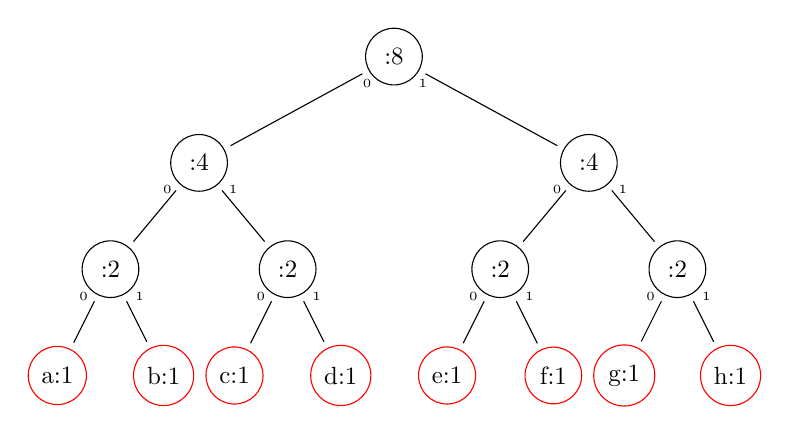
\begin{tikzpicture}[
    scale=0.9,
    transform shape,
    level distance=1.5cm,
    level 1/.style={sibling distance=5.5cm},
    level 2/.style={sibling distance=2.5cm},
    level 3/.style={sibling distance=1.5cm},
    code label/.style={
        font=\tiny\strut,
        inner sep=0pt,
        text width=2.5pt,
        minimum height=0pt,
        anchor=center
    },
    every node/.style={
        draw, 
        circle, 
        minimum size=0.8cm,
        outer sep=0.5pt % Small buffer for perfect edge connection
    },
    edge from parent/.style={
        draw,
        shorten >=0.8mm, % Optimal stopping distance
        shorten <=0.8mm
    }
]
    
    \node[label={[code label,xshift=-2.8pt,yshift=-2.8pt]-135:0},
          label={[code label,xshift=2.8pt,yshift=-2.8pt]-45:1}] (root) {:8}
        child {
            node[label={[code label,xshift=-4.8pt,yshift=-2.8pt]-135:0},
                 label={[code label,xshift=4.8pt,yshift=-2.8pt]-45:1}] {:4}
                child {
                    node[label={[code label,xshift=-2.8pt,yshift=-2.8pt]-135:0},
                         label={[code label,xshift=2.8pt,yshift=-2.8pt]-45:1}] {:2}
                        child { node [draw=red] (a) {a:1} }
                        child { node [draw=red] (b) {b:1} }
                }
                child {
                    node[label={[code label,xshift=-2.8pt,yshift=-2.8pt]-135:0},
                         label={[code label,xshift=2.8pt,yshift=-2.8pt]-45:1}] {:2}
                        child { node [draw=red] (c) {c:1} }
                        child { node [draw=red] (d) {d:1} }
                }
        }
        child {
            node[label={[code label,xshift=-4.8pt,yshift=-2.8pt]-135:0},
                 label={[code label,xshift=4.8pt,yshift=-2.8pt]-45:1}] {:4}
                child {
                    node[label={[code label,xshift=-2.8pt,yshift=-2.8pt]-135:0},
                         label={[code label,xshift=2.8pt,yshift=-2.8pt]-45:1}] {:2}
                        child { node [draw=red] (e) {e:1} }
                        child { node [draw=red] (f) {f:1} }
                }
                child {
                    node[label={[code label,xshift=-2.8pt,yshift=-2.8pt]-135:0},
                         label={[code label,xshift=2.8pt,yshift=-2.8pt]-45:1}] {:2}
                        child { node [draw=red] (g) {g:1} }
                        child { node [draw=red] (h) {h:1} }
                }
        };
\end{tikzpicture}
\end{frame}

\begin{frame}
    \frametitle{\textcolor{myMaroon}{Equal Frequency Huffmans Compression}}
    \begin{itemize}
        \item As we can see if the frequency of the characters is equal then there are no longer or shorter codes

        \vspace{0.4cm}
        \item All encodings are of the same length, a = 000 , f = 101 and etc

        \vspace{0.4cm}
        \item Thus it is not optimal to use huffmans compression for randomly generated strings or when frequency of characters is same because it provides negligible compression
    \end{itemize}
\end{frame}


\begin{frame}
    \frametitle{\textcolor{myMaroon}{Huffman Encoding Table}}
    
    \begin{center}
        \begin{tabular}{c c c}
            \toprule
            \textcolor{myMaroon}{\textbf{Character/Node}} & 
            \textcolor{myMaroon}{\textbf{Frequency}} & 
            \textcolor{myMaroon}{\textbf{Huffman Code}} \\
            \midrule
            a & 1 & 000 \\[0.2cm]
            b & 1 & 001 \\[0.2cm]
            c & 1 & 010 \\[0.2cm]
            d & 1 & 011 \\[0.2cm]
            e & 1 & 100 \\[0.2cm]
            f & 1 & 101\\[0.2cm]
            g & 1 & 110 \\[0.2cm]
            h & 1 & 111 \\[0.2cm]
            
            \bottomrule
        \end{tabular}
    \end{center}
\end{frame}







\begin{frame}
    \frametitle{\textcolor{myMaroon}Question}

    \begin{center}
        \begin{tcolorbox}[
            colback=gray!10,
            colframe=black!60,
            boxrule=0.5pt,
            width=9.5cm,
            halign=left
        ]
            \small
            \textbf{Q. What if the frequency of the characters is an arithmetic progression during Huffman's compression?}
        \end{tcolorbox}
    \end{center}

    % Footer
\end{frame}


\begin{frame}
    \frametitle{\textcolor{myMaroon}{Floyd-Warshall Algorithm}}
    \begin{center}
        {\Large \textbf{\textcolor{myMaroon}{Floyd-Warshall Algorithm}}} \\
        \vspace{0.3cm}
        {\large \textcolor{myBlue}{(Dynamic Programming)}}
    \end{center}

    % Footer
\end{frame}

\begin{frame}
    \frametitle{\textcolor{myMaroon}{Dynamic Programming}}
    \begin{itemize}
        \item A method for solving complex problems by breaking them down into simpler subproblems.

        \vspace{0.4cm}
        \item Stores the results of subproblems to avoid redundant computations (memoization or tabulation).

        \vspace{0.4cm}
        \item Widely used in algorithms like:
        \begin{itemize}
            \item Fibonacci Number Calculation
            \item Matrix Chain Multiplication
            \item Longest Common Subsequence
            \item Floyd-Warshall Algorithm
        \end{itemize}
    \end{itemize}
\end{frame}


\begin{frame}
    \frametitle{\textcolor{myMaroon}{Floyd-Warshall Algorithm}}
    \begin{itemize}
        \item The Floyd-Warshall algorithm is used to find the shortest paths between all pairs of vertices in a weighted graph.

        \vspace{0.4cm}
        \item It uses a dynamic programming approach by progressively improving an estimate of the shortest path between two vertices.

        \vspace{0.4cm}
        \item The core idea is to check whether a path from $i$ to $j$ through an intermediate vertex $k$ is shorter than the previously known shortest path.
    \end{itemize}
\end{frame}

\begin{frame}
    \frametitle{\textcolor{myMaroon}{Floyd-Warshall Algorithm}}
    \begin{itemize}
        \item It can be used to find the shortest path between two nodes in a graph which has negative weight edges

        \vspace{0.4cm}
        \item \textbf{Input: } Graph G

        \vspace{0.4cm}
        \item \textbf{Output: } Shortest path between all nodes.

        \vspace{0.4cm}
        \item \textbf{Time Complexity: } The algorithm runs in \textbf{$\mathcal{O}(n^3)$} time
    \end{itemize}
\end{frame}


\begin{frame}
    \frametitle{\textcolor{myMaroon}{Floyd-Warshall Algorithm}}
    \centering
    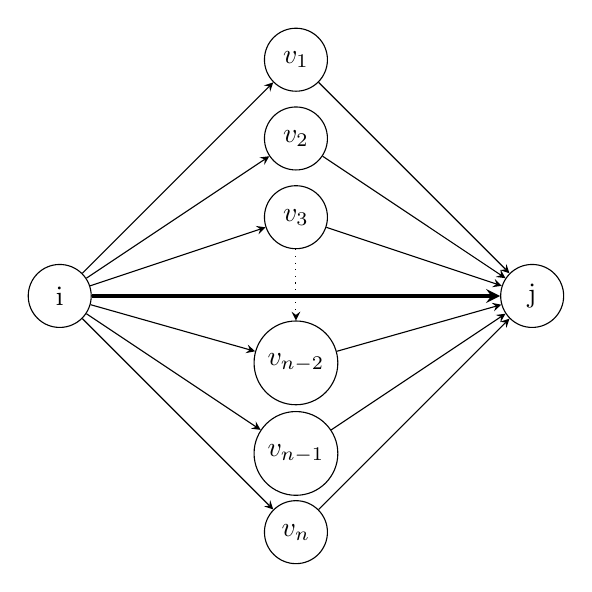
\begin{tikzpicture}[->, >=stealth, auto, node distance=1.2cm,
                        every node/.style={circle, draw, minimum size=0.8cm}]

        % Main nodes
        \node (i) at (0,0) {i};
        \node (j) at (6,0) {j};

        % Intermediate nodes in a vertical column
        \node (v1) at (3,3) {$v_1$};
        \node (v2) at (3,2) {$v_2$};
        \node (v3) at (3,1) {$v_3$};
        \node (v4) at (3,-0.85) {$v_{n-2}$}; % <-- Updated here
        \node (v5) at (3,-2) {$v_{n-1}$}; % <-- Updated here
        \node (vn) at (3,-3) {$v_n$};

        % Edges from s to v's
        \draw (i) -- (v1);
        \draw (i) -- (v2);
        \draw (i) -- (v3);
        \draw (i) -- (v4);
        \draw (i) -- (v5);
        \draw (i) -- (vn);

        % Edges from v's to t
        \draw (v1) -- (j);
        \draw (v2) -- (j);
        \draw (v3) -- (j);
        \draw (v4) -- (j);
        \draw (v5) -- (j);
        \draw (vn) -- (j);

        % Direct edge from s to t
        \draw[very thick] (i) -- (j);

        \draw[dotted] (v3) -- (v4);

    \end{tikzpicture}
\end{frame}

\begin{frame}
    \frametitle{\textcolor{myMaroon}{Floyd-Warshall Algorithm}}
    \begin{itemize}
        \item As we can see there are total n-1 paths from i to j

        \vspace{0.4cm}
        \item d(i$\rightarrow$j)

        \vspace{0.4cm}
        \item d(i$\rightarrow$$v_k$) + d($v_k$$\rightarrow$j)

        \vspace{0.4cm}
        \item The shortest possible path between i and j will be the one with the one with the minimum distance from these paths 
    \end{itemize}
\end{frame}


\begin{frame}
    \frametitle{\textcolor{myMaroon}{Floyd-Warshall Algorithm (Dynamic Programming)}}
    \begin{itemize}
        \item d(i,j,n) will provide the shortest possible path between nodes i and j (where n is total number of vertices in the graph).

        \vspace{0.4cm}
        \item Let d(i,j,k) be the shortest path between nodes i and j which allows traversal of first K nodes within the graph.

        \vspace{0.4cm}
        \item We can determine d(i,j,k+1) from d(i,j,k) such as,

        \vspace{0.4cm}
        \item
        d(i,j,k+1) = MIN (d(i,j,k), d(i,k+1,k) + d(k+1,j,k))
    \end{itemize}
\end{frame}

\begin{frame}
    \frametitle{\textcolor{myMaroon}HomeWork}

    \begin{center}
        \begin{tcolorbox}[
            colback=gray!10,
            colframe=black!60,
            boxrule=0.5pt,
            width=9.5cm,
            halign=left
        ]
            \small
            \textbf{Q. Implement a dynamic array in C++ and analyze the amortized cost of its insertions.}
        \end{tcolorbox}
    \end{center}

    % Footer
\end{frame}

\end{document}